\section{Static Single Assignment}

In this lecture we will cover what is SSA and how to convert a program to SSA form.

\subsection{}

When we are trying to do some types of optimizations, it is often nice to know when is a variable is defined.
For loop invariant code motion where we are trying to move computations outside of a loop, you will see it is very important to 
know where the definitions are.



Take the code\ref{fig:ssaexm1} for example, if \texttt{B,C,D} are defined outside the loop, we can move the computation ouside the loop.

% \begin{figure}[h]
%     \centering
%     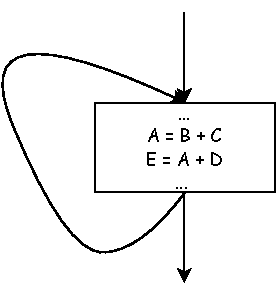
\includegraphics[width=0.4\textwidth]{ssaexm1.drawio.pdf}
%     \caption{Example of Loop-Invariant Code Motion}
%     \label{fig:ssaexm1}
% \end{figure}


Copy optimization is also an important optimization and one way that you can do some analysis for copy propogation is that you can 
look for any use of a variable if it turns out that all of the reaching definitions of it are of the form where they are coping the same 
variable. Take the code \ref{fig:ssaexm2} for example. If all reaching definitions of \texttt{X} copies the same variable \texttt{Y}, and \texttt{Y} is not 
redefined since that copy, then we can substitute use of \texttt{X} with use of \texttt{Y} and then hopefully the assigment \texttt{X = Y} will end up becoming dead code later.

It's often nice to know the relationship between when variables are used and when they are defined. So the motivation for SSA is that it would be nice to directly traverse between definitions and uses 
between definitions and uses for paticular variables instead of having to look everything that is going on inside a flow graph. Argubly this will not only be convinient but also it might make things more efficient becuase I 
can jump over all the instructions irrelevant to the analysis that I am doing. Another insight is that sometimes variables get reused but if we're overwriting a variable in the second time, the later 
uses may have nothing to do with earlier uses and definitions of the variable. So specifically, \texttt{X} appears twice in the CFG, but the definition and use of \texttt{X} actually have nothing to do with that in the second block.
So considering them to be the same variable is going to inhibit optimizations potentially. It would be nice if the compiler could realize they are seperate variables effectively.


One way that you could potentially deal with wanting to go directly between uses and definitions is to create a type of index or a data structure called Definition-Use or Use-Definition chains. But it has a downside which means the chains can be expensive.

In the case , if we even just consider one definition and all its uses, or one use and all of its definitions, these data structures can be non-trivially large. In general, if you have N definitions and M uses, the complexity of time and memory is \texttt{O(MN)}. 


% \begin{figure}[h]
%     \centering
%     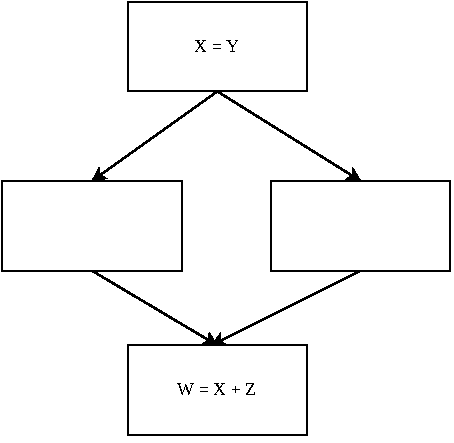
\includegraphics[width=0.4\textwidth]{ssaexm2.drawio.pdf}
%     \caption{Example of Copy Propogation}
%     \label{fig:ssaexm2}
% \end{figure}
% \subsection{The Development of Static Single Assignment Form}




\begin{figure}[h]
    \centering
    \begin{subfigure}[b]{0.4\textwidth}
        \centering
        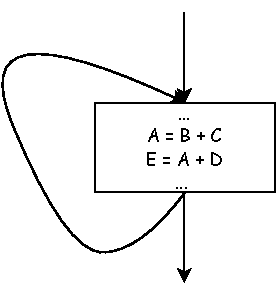
\includegraphics[width=0.6\textwidth]{ssaexm1.drawio.pdf}
        \caption{Example of Loop-Invariant Code Motion}
        \label{fig:ssaexm1}
    \end{subfigure}
    \hfill
    \begin{subfigure}[b]{0.4\textwidth}
        \centering
        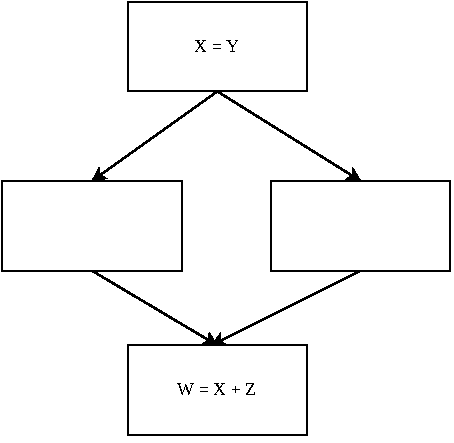
\includegraphics[width=0.6\textwidth]{ssaexm2.drawio.pdf}
        \caption{Example of Copy Propogation}
        \label{fig:ssaexm2}
    \end{subfigure}
      
    \caption{two examples}
\end{figure}




This concept is based on \footnote{\url{https://compilers.cs.uni-saarland.de/ssasem/talks/Kenneth.Zadeck.pdf}}


In the very Beginning, there was dataflow analysis.   Ultimately dataflow analysis turns out to be very expensive.

Viewing the program variable by variable exposes structure that is obscured by the dataflow model: 
A kill allows the cfg to be clipped. Also, the dataflow for a single variable can be solved
without iteration. This turns out to be a dead end, but it set the
stage for the development of SSA.


Take constant propogation for example, Kildall and Wegbreit use a conventional
dataflow framework. The fact vector is very large: values not bits. Must use iteration.
The time to run these is between \(O(ElogEV)\) and
\(O(E^2 V)\) depending on the type of control flow
graph processing.



\subsubsection{The First Attack}


Use def-use chains. Sometimes this helps and sometimes it does not. This requires NMV
def-use chains.

\begin{lstlisting}[language=C,frame=single, caption=An ,label = lst:expr2]
switch (...) {
case 1: x=...; y=...; break;
...
case n: x=...; y=...; break;
}
switch (...) {
case 1: ...=x; ...=y; break;
...
case m: ...=x; ...=y; break;
}
\end{lstlisting}


\subsubsection{The Second Attack }


Add a “join birthpoint”
for x and y between
the two switches. 



\begin{lstlisting}[language=C,frame=single, caption=An ,label = lst:expr2]
    switch (...) {
    case 1: x=...; y=...; break;
    ...
    case n: x=...; y=...; break;
    }
    birthpoint x, y;
    switch (...) {
    case 1: ...=x; ...=y; break;
    ...
    case m: ...=x; ...=y; break;
    }
    \end{lstlisting}